\section{Overview}
\section{Br\'eguet's Range Equation}
\hspace{.5cm} Br\'eguet's range equation used as an objective function according to \cite{breguetRangeEqn}, shown in Eq. \ref{eqBreguet}, combines specific fuel consumption in kilograms per horsepower-hour, lift, drag, cruising speed, and initial and final fuel weights with aircraft weight. The derivation of this equation starts with several steps that are important for the sake of assumptions used in each simplification. Eq. \ref{eqRangeEq} is integration over the change in weight to solve for distance. 
\begin{equation}
    R = \int_{W_1}^{W_0}\dfrac{VdW}{(TSFC)D}
    \label{eqRangeEq}
\end{equation}
Assuming constant altitude, constant angle-of-attack, and constant thrust specific fuel consumption, the equation simplifies to Eq. \ref{eqBreguet}.
\begin{equation}
\label{eqBreguet}
R = \sqrt{\dfrac{2}{\rho_\infty S}}\left(\dfrac{1}{TSFC}\right) \left(\dfrac{C_L^{1/2}}{C_D}\right)(\sqrt{W_0}-\sqrt{W_1})
\end{equation}
The simplicity of this equation lends itself well to optimization of more complex problems. Taking away the assumption for constant altitude and assuming a constant airspeed, the equation uses less constants involving density and becomes Eq. \ref{eqAirspeedAOA}.
\begin{equation}
\label{eqAirspeedAOA}
    R = \dfrac{V}{TSFC}\left(\dfrac{C_L}{C_D}\right)\ln\dfrac{W_0}{W_1}
\end{equation}
\cite{fuelsLOGRange} uses this equation to compare fuel design effects on range. \par
The final well-established derivation of the range equation is the equation assuming a constant airspeed, constant altitude, and parabolic drag polar. Eq. \ref{eqDragPolar} shows the result of these assumptions on Eq. \ref{eqRangeEq}.
\begin{equation}
\label{eqDragPolar}
    R = \dfrac{2V}{TSFC}\left(\dfrac{L}{D}\right)_{max}\left[\tan^{-1}\dfrac{C_{L_1}}{C_{L_{md}}}-\tan^{-1}\dfrac{C_{L_2}}{C_{L_{md}}}\right]
\end{equation}
The main limitation of aeronautics overall is the ability to project an aircraft into future space due to three common dependent factors of thrust, lift, and drag.\par
Lift and drag are simplified when trying to maximize lift and drag. Eqs. \ref{eq:maxlift} and \ref{eq:maxdrag} illustrate these simplifications as shown in the basic performance equation introduced by \cite{OptimizeBreguet}.
\begin{equation}
C_{L_{MR}} = \sqrt{\dfrac{C_{D_0}}{3\epsilon}}
\label{eq:maxlift}
\end{equation}
\begin{equation}
C_{D_{MR}} = \dfrac{4}{3}C_{D_0}
\label{eq:maxdrag}
\end{equation}
\par
\cite{Jonas1947} argues that these equations are not accurate at predicting realistic results when accounting for change in weight over time changes the fuel efficiency of the aircraft. The new derivation of a range equation where weight is dynamic gave the following equation.
\begin{equation}
    R = (b/a)[\arctan(W_i/a)-\arctan(W_f/a)].
    \label{eq:dynamicrange}
\end{equation}
The constants $a^2$ and $b$ are given by 
\begin{equation}
    \begin{aligned}
        a^2 &= \dfrac{C_0qS+C_1C_{D_0}(qS)^2}{\epsilon C_1}\\
        b &= \dfrac{VqS}{\epsilon C_1}
    \end{aligned}
\end{equation}
where $C_0$ and $C_1$ are constants for altitude and airspeed. The results of these derivations were applied to a hypothetical jet. The results showed a range only 0.77\% higher than the exact value obtained from the original range equation. The eventual argument for the new method was convenience of aircraft and engine parameters available. With the assumptions for each derivation of Br\'eguet's range equation, the resulting equations are accurate and new methods are even compared to the results of these equations for accuracy.\par
As stated before, the weight change over time changes the fuel efficiency of an aircraft. \cite{Jonas1947} derives an equation involving the overall efficiency slope, $m$ that describes fuel efficiency. Eq. \ref{eqRangeIncludesM} shows the results of this derivation.
\begin{equation}
    R = \dfrac{aVJC_H}{10,560m}log_e\dfrac{W_i}{W_i-W_F}
    \label{eqRangeIncludesM}
\end{equation}
where $V$ is airspeed in ft. per sec., $J$ is a constant representing mechanical heat at 778.26 ft.lbs. per B.t.u., and $C_H$ is the fuel heat value in B.t.u. per lb. $a$ is equivalent to $2C_L/C_D$. These values are more difficult to acquire and so the most useful equation was derived by \cite{Jonas1947} shown in Eq. \ref{RangeChanges}.
\begin{equation}
    R = \dfrac{W_i}{1.467}\dfrac{V}{Q_I}log_e\dfrac{W_i}{W_i-W_f}
    \label{RangeChanges}
\end{equation}
where $Q_I$ is $\theta_f/\theta_i$ which is the ratio of altitude density over the course of the cruise. This equation is useful when reducing the amount of assumptions in a flight plan. Eqs. \ref{RangeChanges} and \ref{eqRangeIncludesM} get rid of the assumption of constant altitude.\par
\section{Endurance Equation}
In addition to maximum range, loiter time is needed and relates to the endurance equation. Endurance is the calculated time that an aircraft can remain in the air. Eq. \ref{endure} shows the calculation.
\begin{equation}
\label{endure}
E = \dfrac{1}{TSFC}\left(\dfrac{L}{D}\right) \ln\left(\dfrac{W_i}{W_f}\right)
\end{equation}
The endurance equation's lift and drag elements can be replaced by an angle of attack for best endurance \cite{OptimizeBreguet} shown in equation \ref{eq:maxendurance}.
\begin{equation}
\label{eq:maxendurance}
\dfrac{L}{D} = \dfrac{C_{L_{ME}}}{C_{D_{ME}}} = \sqrt{\dfrac{1}{4KC_{D_0}}}
\end{equation}
\par 
The simplification of these equations involves introducing an unknown amount of error into a continuous problem. There are analytical solutions to reducing this error shown in \cite{OptimizeBreguet} and \cite{LoiterTimeFromRange}. These can be incorporated and tested against the existing high-fidelity solutions.\par

\section{Thrust Relations}

\section{Multiobjective Optimization}
Pareto introduced the concept of dominated solutions in the field of economics in 1906 to describe a solution that best serves all parties in a multiplayer game \cite{paretomanual}. Now, science and engineering have coordinated this concept into design and performance optimization \cite{surveyMarler}. A Pareto Frontier in an aircraft's performance space can be easily visualized when there are few objectives. In this case, two objectives gives a reasonable expectation for a straightforward visualization. \cite{MultiobjectiveVisualization} uses an initial mapping from a design space to a performance space in multiple dimensions and proves that the visualization using performance is a better method for an $n$-dimensional design space. The performance space of the Pareto Frontier proposed in this paper is only two dimensional and does not require the complicated mapping of a design space to a performance space from multiple dimensions.\par
Multi-objective optimization with two objectives and two performance variables can be seen in Eqs. \ref{eq:exfunction1} and \ref{eq:exfunction2}.
\begin{align}
    f_1(x) &= \sqrt{1+x^2}\label{eq:exfunction1}\\
    f_2(x) &= 4+2*\sqrt{1+(x-1)^2}
    \label{eq:exfunction2}
\end{align}
$f_1(x)$ is increasing as $f_2(x)$ is decreasing between zero and one so there is a tradeoff region between the two functions in optimization. Figure \ref{visualex} shows the tradeoff region for the two functions.

\begin{figure}%
    \centering
    \label{visualex}
    \subfloat[Plot of two objective functions.]{{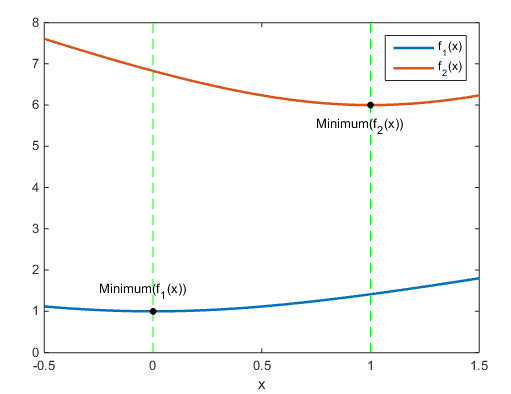
\includegraphics[width=7cm]{Thesis/LiteratureReview/VisualExTwoObj.png} }}%
    \qquad
    \subfloat[Tradeoff region due to weighted optimization.]{{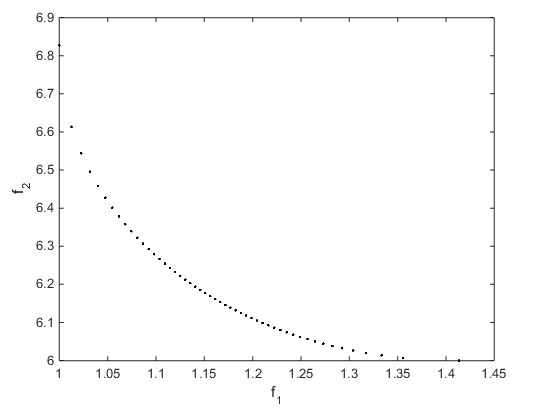
\includegraphics[width=7cm]{Thesis/LiteratureReview/VisualExTradeoff.png} }}%
    \caption{Example of a weighted Pareto Frontier.}%
    %
\end{figure}

By using multi-objective optimization, the Pareto Frontier shows the optimums given that one function is more important than another over this tradeoff region. Figure \ref{fig:tradeoffex} shows the tradeoff between the two objectives.


\par
\cite{MultOptCS} points out that there are two main methods when approaching a multiobjective optimization problem. These are the weighting method and the constraint method. In these two methods, the decision maker can control the solution process with their preferences.\par
\subsection{Weighting Method}
The weighting method involves solving the following multiobjective optimization problem,
\begin{equation}
\begin{aligned}
    & minimize \sum^k_{i=1} w_if_i(\mathbf{x})\\
    & subject \ to \ \mathbf{x}\in S,
\end{aligned}
\label{eq:weightEq}
\end{equation}
where $w_i\geq 0 \ \ \forall i = 1,\dots,k$ and each objective is normalized so that magnitudes are not a factor in the solutions. The solution to Eq. \ref{eq:weightEq} is weakly Pareto optimal, meaning that the solution is not necessarily unique. The solution is Pareto optimal if for all $i = 1,\dots,k$, $w_i>0$ or if the solution is unique \cite{MultOptCS}. The weighting method can be used as a decision tool to generate different Pareto optimal solutions for the decision maker to choose from. The main requirement for the use of a weighting method is a convex problem. The optimal solutions of some nonconvex problems can sometimes be found no matter the weights, but cannot be proven and does not always behave like the convex solution method \cite{MultOptCS}.\par
\subsection{$\epsilon$-Constraint Method}
The second method is the $\epsilon$-constraint method where one of the objective functions is selected to be optimized and the rest are used as constraints in the optimization problem. The form of this problem can be seen in Eq. \ref{eq:constraintEq}.
\begin{equation}
    \begin{aligned}
    \text{minimize} \ & f_i(\mathbf{x})\\
    \text{subject to} \ & f_j(\mathbf{x})\leq \epsilon_j \ \forall j = 1,\dots,k, \ j\neq l,\\
    & \mathbf{x}\in S.
    \end{aligned}
    \label{eq:constraintEq}
\end{equation}

\section{Conclusion}
